% InsPLAD-QA paper draft (English). Compile with pdfLaTeX + BibTeX (e.g. Overleaf).
% Numbers come from the repository result files cited in each table source comment.
% Matched-call control filled from run 902a9f8a1752 (reports/gold_matched_call_evaluation_2026-10-23), CPU-audited.
\documentclass[11pt]{article}
\usepackage[margin=1in]{geometry}
\usepackage[T1]{fontenc}
\usepackage{lmodern}
\usepackage{amsmath}
\usepackage{booktabs}
\usepackage{graphicx}
\usepackage{multirow}
\usepackage{xcolor}
\usepackage{url}
\usepackage[numbers,sort&compress]{natbib}
\usepackage[hidelinks]{hyperref}

\newcommand{\TBD}{\textcolor{red}{TBD}}
\newcommand{\CondImg}{Image only}
\newcommand{\CondNorm}{+ normal ref.}
\newcommand{\CondPos}{+ defect ref.}
\newcommand{\CondBoth}{+ normal \& defect ref.}
\newcommand{\CondVX}{+ vision expert (mean of 20)}

\title{InsPLAD-QA: Benchmarking Vision-Language Models\\
and a Verification Agent for Power-Line Inspection}
\author{Anonymous authors}
\date{}

\begin{document}
\maketitle

\begin{abstract}
Large vision-language models (LVLMs) are increasingly proposed as zero-shot inspectors, yet no power-line inspection benchmark tests whether they detect a defect, name it, and answer consistently. We build \emph{InsPLAD-QA}, an MMAD-style question-answering benchmark on the public InsPLAD UAV dataset. We align its two releases by exact image hashes and freeze a manually reviewed gold set of 246 images and 534 questions. Four open LVLMs and one API pipeline share one prompt, output schema and evaluator; the open models are also tested with a normal reference, a defect reference, both, and 20 vision-expert cues. A normal reference raises anomaly-detection F1 for every open model, but balanced accuracy rises clearly for only two of them, and MiniCPM-V-4.5's falls (.656 $\rightarrow$ .587) because it flags most normal images. Expert cues mostly raise defect-type F1 and lower anomaly-detection F1. A question-independent verification agent, chosen on a disjoint development set and run once on gold, raises the macro-F1 of the four-way type question, which includes ``normal'', from .522 to .640 (paired 95\% CI of the gain $[+.043,+.199]$). Of its 27 additional correct answers, 23 are on normal images; on the 139 defective images correct types rise only from 93 to 97. The agent's staged region question cuts false regions on normal images from 93/107 to 16/107 and misses 27/139 defects instead of 4/139, but the direct region question it is compared with reports a region on almost every image. Against the model's own binary question (17 false alarms, 40 misses) the staged answer is better on both counts, and it locates defects no better than a constant ``center'' answer. An equal-call re-ask without the agent's definitions and staging trails it by .164 macro-F1 and .203 presence BAcc (both CIs exclude zero), so extra calls do not explain the gain. Missing insulator caps are the main failure: the binary question flags 3 of 27 and the staged region question 9. On development data, higher resolution, other LVLMs, anomaly detectors and part-evidence tools did not reliably recover them, and InternVL3.5-8B did not report them on crops of the annotated location. An asset-specific supervised classifier detected all 25 development missing caps, although these images may share capture dates with its training data. We release the benchmark, code and per-question answers, and recommend that inspection benchmarks report false alarms and misses separately and compare each answer with constant baselines.
\end{abstract}

\section{Introduction}
Utilities inspect thousands of kilometres of transmission line with unmanned aerial vehicles (UAVs), and the resulting images are reviewed largely by hand. LVLMs promise to answer open questions about such images without task-specific training. Industrial anomaly-detection benchmarks for LVLMs, notably MMAD~\cite{jiang2025mmad}, show that general models still lag behind human inspectors on manufactured objects. Power-line assets differ from bench-top industrial objects: they are photographed outdoors from varying viewpoints, against cluttered backgrounds, and their defects range from surface rust to entirely missing components.

This paper asks three questions. (i) How well do current open LVLMs detect and classify defects on power-line assets under a fair, shared contract? (ii) Do a normal reference image or anomaly-detector (``vision expert'') cues help? (iii) Does a training-free verification agent improve the answers, and at what cost? The agent re-examines each question separately. For the defect type it adds option definitions and the question's own earlier answer, and for the defect region it asks a presence question before a position question.

Our contributions are:
\begin{itemize}
  \item \textbf{InsPLAD-QA}, a reproducible benchmark built from InsPLAD~\cite{vieira2023insplad}. It has two tracks, an exact-hash \emph{Aligned Core} of 1,378 images shared by both releases, and a manually reviewed, frozen gold set (246 images, 534 questions). Leakage controls cover reference selection and the development split (Section~\ref{sec:benchmark}).
  \item A controlled comparison of four open LVLMs and an API pipeline under identical prompts, schema and scoring. All five are tested image-only. Each of the four open models is also tested with normal, defect and combined references and with 20 vision-expert configurations. We report consistency between questions as well as accuracy (Section~\ref{sec:baselines}).
  \item A question-independent verification agent, selected on a disjoint development set and evaluated once on gold. It improves the four-way type answer, although 23 of its 27 additional correct answers are on normal images, and its staged region-presence answer has fewer false alarms and fewer misses than the model's own binary answer. It does not locate defects better (Section~\ref{sec:agent}). A matched-call control, which re-asks with the same number of calls but without definitions or staging, does not reproduce the gain and shifts answers towards ``normal''.
  \item An analysis of missing-component defects, which no question detects reliably. On development data, training-free interventions did not recover them, and InternVL3.5-8B did not report them even when shown a crop of the annotated location (Section~\ref{sec:missing}).
\end{itemize}

\section{Related Work}
\paragraph{Power-line inspection.} Utilities increasingly inspect transmission lines with UAV images analysed by deep learning~\cite{nguyen2018review}. Public data mostly serve trained, task-specific models. Tao et al.\ detect insulators and their defects in aerial images with cascaded CNNs and release CPLID~\cite{tao2020cplid}. STN PLAD annotates five asset types for multi-size detection in high-resolution UAV images~\cite{vieira2021stnplad}, and InsPLAD adds anomaly-detection and fault-classification splits over 17 asset types~\cite{vieira2023insplad}. None of them asks whether a general LVLM can detect, name and consistently describe a defect, which is what InsPLAD-QA tests.

\paragraph{LVLMs for industrial anomaly detection.} AnomalyGPT~\cite{gu2024anomalygpt} fine-tunes an LVLM with simulated anomalies, while MMAD~\cite{jiang2025mmad} benchmarks general LVLMs with multiple-choice questions on industrial objects. MMAD also studies agent-style aids such as expert anomaly maps and retrieved domain knowledge. We adopt MMAD's question format and its normal-reference (one-shot) setting, apply them to power-line UAV imagery, and add explicit cross-question consistency metrics.

\paragraph{Anomaly detectors as experts.} We give the LVLMs cues from four unsupervised detectors and chose one from each of four families, so that a cue effect is not tied to one design. PatchCore~\cite{roth2022patchcore} keeps pretrained patch features of normal images in a memory bank and scores a patch by its nearest-neighbour distance. ReConPatch~\cite{hyun2024reconpatch} first learns a contrastive projection of those patch features. Dinomaly~\cite{guo2025dinomaly} reconstructs DINO features and trains one model for many object types. AnomalyCLIP~\cite{zhou2024anomalyclip} compares image patches with learned object-agnostic normal and abnormal text prompts and needs no training on the target domain. All four output an image score and an anomaly map, and none uses defect-type labels.

\paragraph{Self-verification.} Iterative self-feedback can improve LLM outputs~\cite{madaan2023selfrefine}, but asking a model to reconsider without new information can also degrade correct answers~\cite{huang2024cannotselfcorrect}. This motivates our matched re-ask control: it spends the same number of calls as the agent but supplies no new evidence.

\section{Benchmark}\label{sec:benchmark}
Figure~\ref{fig:pipeline} summarizes how the benchmark is built and evaluated.

\begin{figure}[t]
\centering
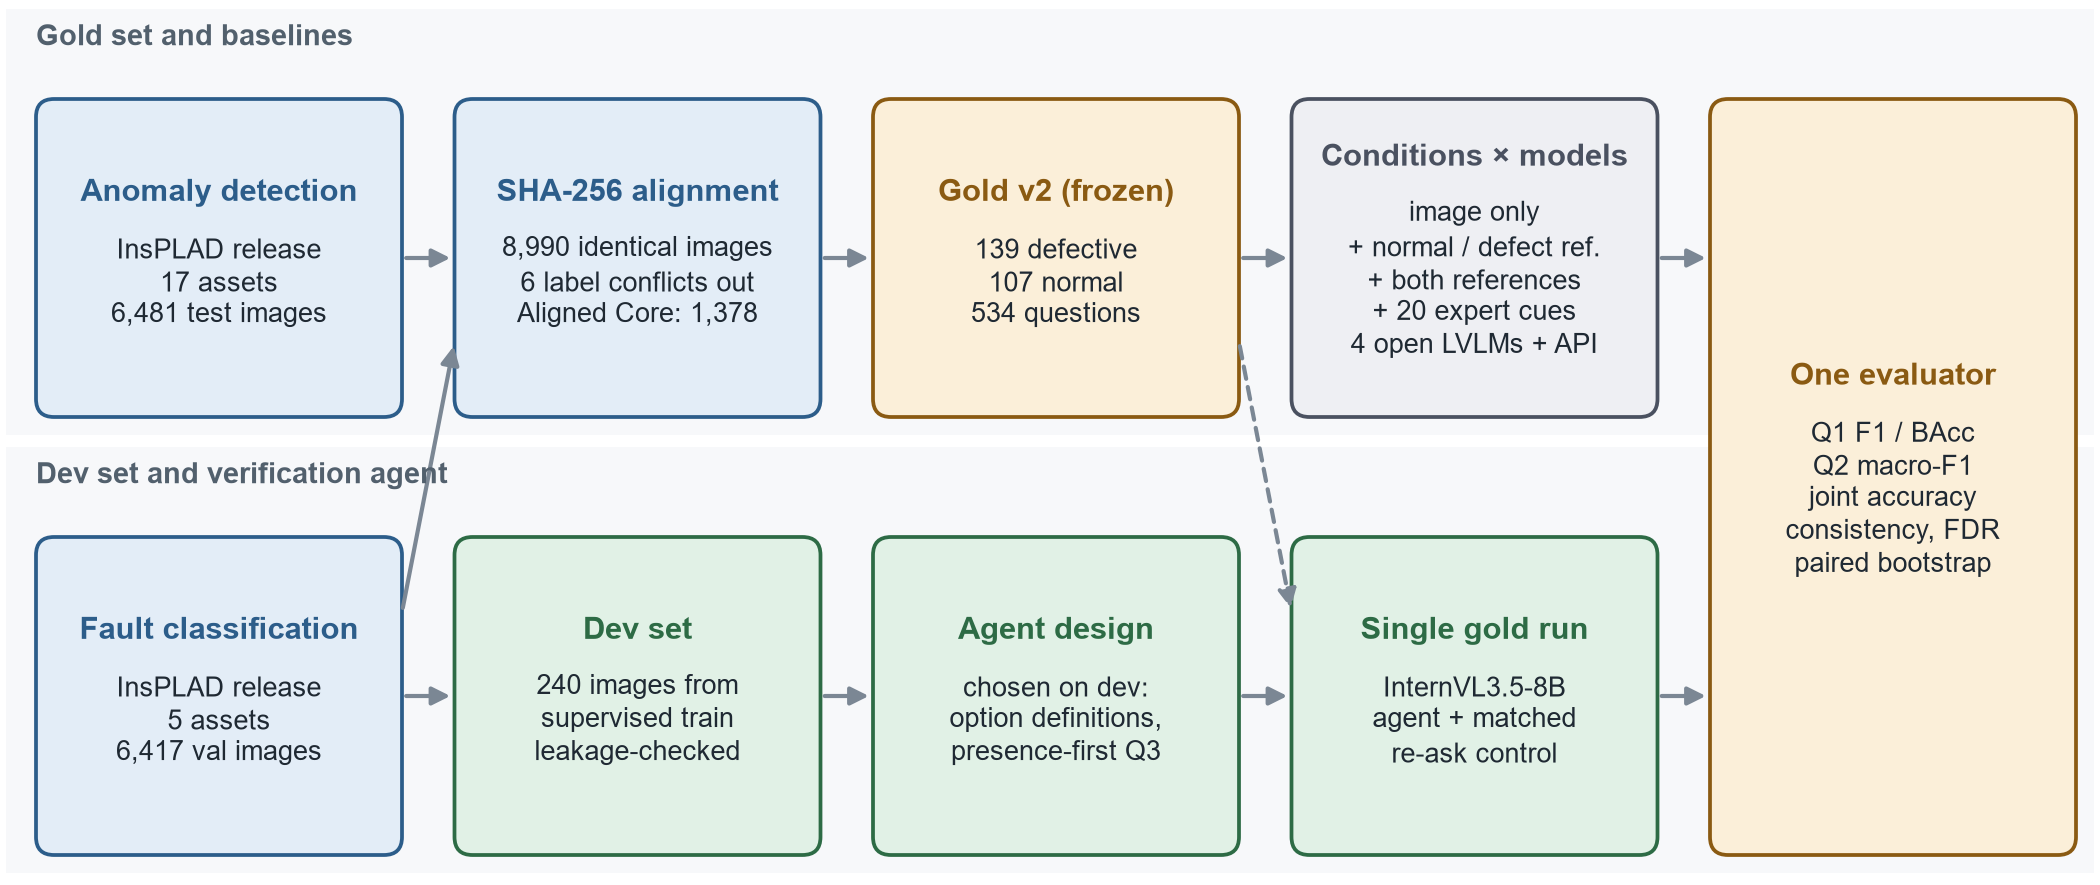
\includegraphics[width=\linewidth]{figures/fig_pipeline_en.png}
\caption{How the benchmark is built and used. Top: the frozen gold set and the baseline comparison. Bottom: the dev set, on which the verification agent is designed before its single gold run.}
\label{fig:pipeline}
\end{figure}

\subsection{Source data and label policy}
InsPLAD~\cite{vieira2023insplad} provides two releases. The unsupervised anomaly-detection release covers 17 asset categories and 27,620 JPEG images split into train and test (6,481 test images). Three of its assets (\texttt{damper-preformed}, \texttt{spacer}, \texttt{yoke}) are normal-only in test. The supervised fault-classification release covers 5 assets and 11,525 images in train and val (6,417 val images); it has no test split. Folders named \texttt{good} or \texttt{normal} map to \emph{normal}, and every defect folder maps to \emph{anomalous}. We only slug-normalize \texttt{corros\~ao} to \texttt{corrosao} and never merge it with \texttt{rust}. The integer IDs in the supervised annotation file are asset-local class indices, not binary labels, so semantic labels come from folder names.

\subsection{Tracks and Aligned Core}
Track~A (general anomaly detection) uses all 6,481 unsupervised test images in zero-shot and one-shot (normal reference) form. Track~B (structured fault understanding) uses the 6,417 supervised val images and asks for both the anomaly label and the defect class. The two releases share 8,990 SHA-256-identical images; 1,384 of them lie in both unsupervised test and supervised val. Six of these carry conflicting binary labels and are excluded, which leaves an \emph{Aligned Core} of 1,378 images. On these images zero-shot, one-shot and structured answers can be compared byte for byte.

\subsection{Gold v2 QA set}
Running every model on every configuration over the full tracks is costly, and several labels needed manual checking. We therefore built a gold set from the Aligned Core: all 139 of its defective images, plus normal images capped per asset at the median and chosen for diversity with DINOv2~\cite{oquab2024dinov2} embeddings. Every image was manually reviewed and none was excluded. The set was then frozen (Table~\ref{tab:gold}). Each image has a binary question (Q1: ``Is the target power-line asset normal or anomalous?'') and a four-way defect-type question (Q2: rust/corrosion, bird nest, missing cap, normal). Forty-two images also carry an MMAD-style four-option localization question (Q3), for 534 questions in total. Option order is fixed per question and independent of the answer. Figure~\ref{fig:qa} shows one gold image per class with its ground truth and the answers of the direct question and the verification agent (Section~\ref{sec:agent}).

\begin{figure}[t]
\centering
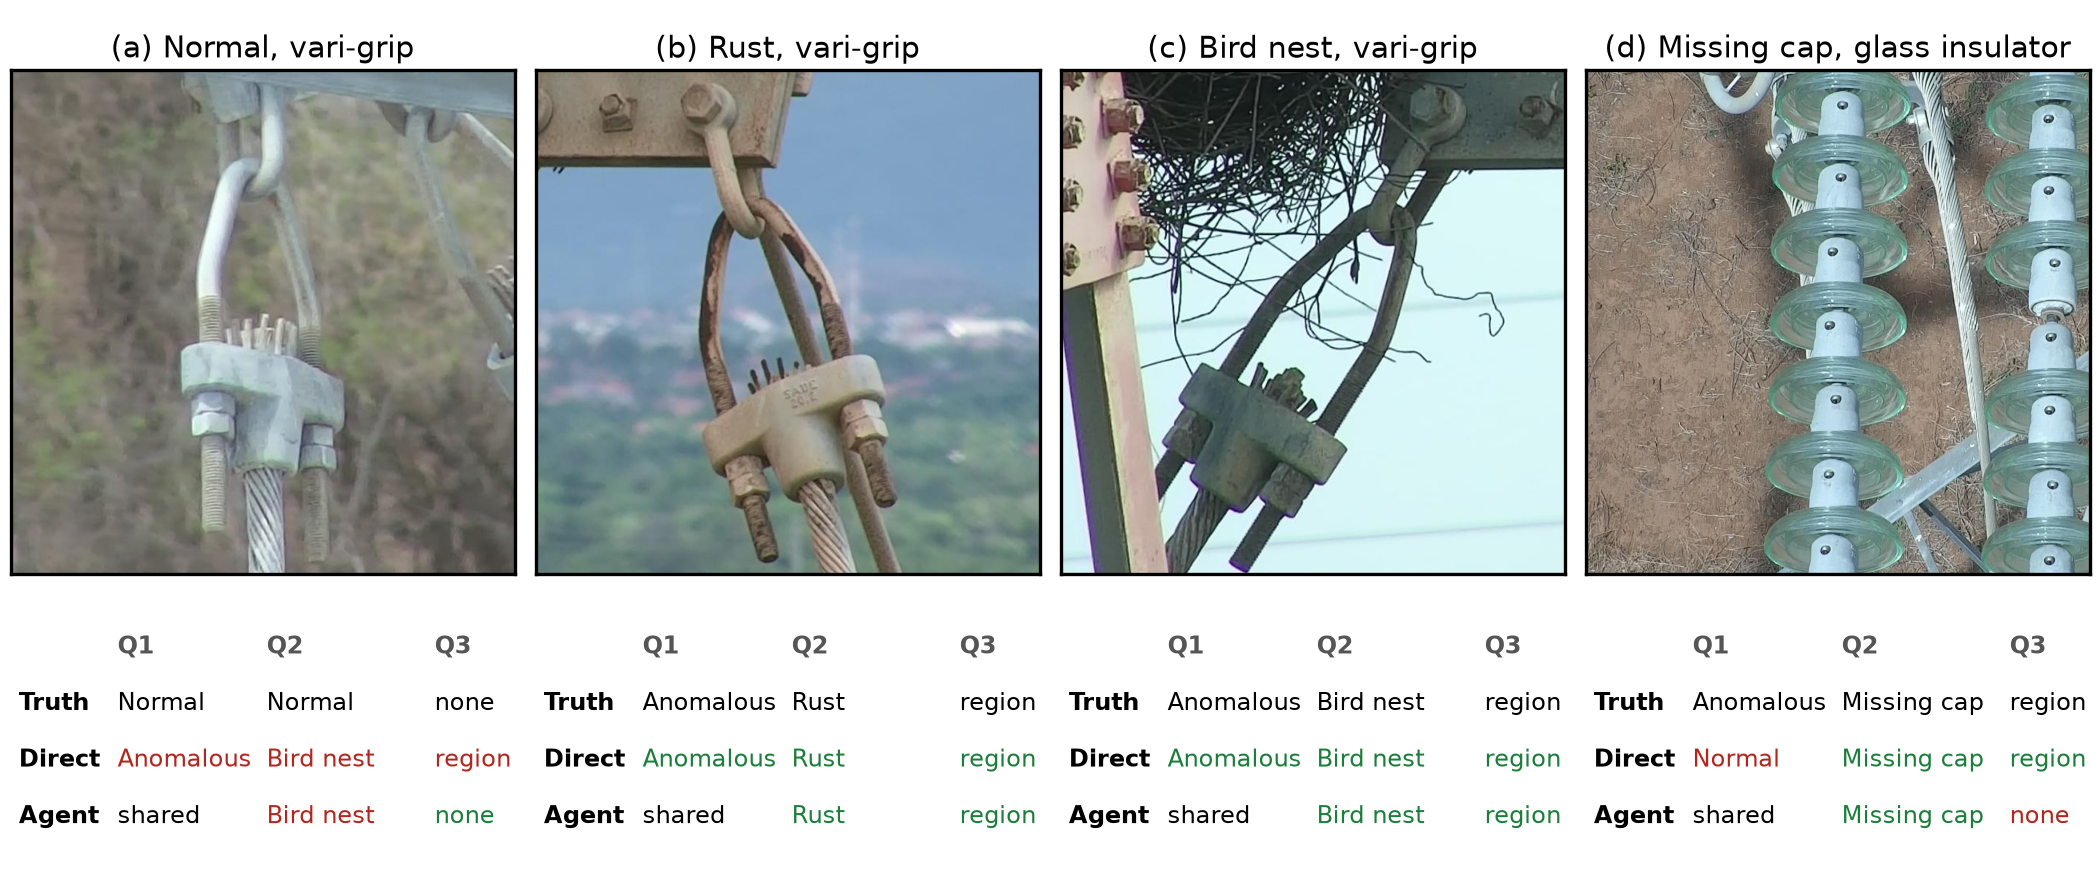
\includegraphics[width=\linewidth]{figures/fig_qa_examples_en.png}
\caption{One gold image per class with ground truth and InternVL3.5-8B answers (green: correct, red: wrong). Q1: ``Is the target power-line asset normal or anomalous?'' Q2: ``Which condition best describes the target power-line asset?'' (normal, rust/corrosion, missing cap, bird nest). Q3 is scored for presence: ``region'' means a defect region was reported. The agent keeps the direct Q1 answer. Its staged Q3 removes the false alarm in (a) but misses the cap in (d). Images: InsPLAD~\cite{vieira2023insplad}, CC BY-NC 3.0.}
\label{fig:qa}
\end{figure}

\begin{table}[t]
\centering
\caption{Frozen gold v2 composition (images). All 27 missing-cap images are glass insulators, an asset with only five normal images.}
\label{tab:gold}
\begin{tabular}{lrrrrr}
\toprule
Asset & Images & Normal & Rust & Bird nest & Missing cap \\
\midrule
% Source: results/latest/gold_v2_final/master_counts.csv and the frozen gold Q2 labels (defect_gt).
glass-insulator                 & 32 & 5  & --  & --  & 27 \\
lightning-rod-suspension        & 53 & 33 & 20  & --  & -- \\
polymer-insulator-upper-shackle & 32 & 3  & 29  & --  & -- \\
vari-grip                       & 76 & 33 & 20  & 23  & -- \\
yoke-suspension                 & 53 & 33 & 20  & --  & -- \\
\midrule
Total                           & 246 & 107 & 89 & 23 & 27 \\

\bottomrule
\end{tabular}
\end{table}

\subsection{Development set and protocol}
Every method choice was made on a separate development set. It has 240 images (480 Q1/Q2 questions; 125 normal, 115 defective) drawn with seed 42 from the supervised \emph{train} split, because the Aligned Core's defective images are all in gold. Dev excludes any image whose size and CRC32 fingerprint occurs in unsupervised test, in a fixed reference, or in gold. Configurations were frozen in a committed file before their single gold run, and gold scores never fed back into configuration choices. Gold had been used for earlier baseline comparisons, so we do not call it an untouched holdout.

\subsection{References and leakage controls}
A one-shot reference is a normal image of the same asset from unsupervised \emph{train}. We exclude any candidate whose fingerprint appears in test. The \emph{fixed} reference is drawn once per asset with seed 42. The \emph{retrieved} reference is the DINOv2-base cosine nearest neighbour of the target (pinned weights). Retrieval exposed a shortcut on dev: normal targets often retrieved a reference from the same capture date (44\% vs.\ 16\% for defective targets), and cosine similarity alone separated normal from defective images with AUROC .886. These numbers are recomputed from the committed dev image list. We therefore exclude same-capture-date candidates (\emph{diffdate}) in every retrieved condition used by the agent.

\subsection{Metrics}
For Q1 we report accuracy and F1; balanced accuracy (BAcc), precision, recall and TP/FP/TN/FN are in the released result files. For Q2 we report accuracy and macro-F1 over the classes present, and the agent tables also report Q2 BAcc (mean recall over the classes present). Q2 has four options including ``normal'', so these scores also reward correct ``normal'' answers on normal images; the agent tables therefore add the number of defective images typed correctly. Invalid outputs count as wrong. For Q1, an invalid answer on a defective image is a false negative. On a normal image it is kept separate from false positives, so it lowers specificity but not precision. \emph{Joint accuracy} counts images where Q1 and Q2 are both correct. \emph{Consistency error} is the share of images with valid answers where Q1 and Q2 disagree (normal with a defect type, or anomalous with ``normal''). \emph{False defect rate} is the share of normal images given a defect type. Differences between policies use a paired bootstrap over images with 2,000 resamples~\cite{efron1994bootstrap}.

\section{Models and Baselines}\label{sec:baselines}
\subsection{Setup}
We keep one model per model line: Qwen3.5-4B~\cite{qwen35} with thinking disabled, InternVL3.5-8B~\cite{wang2025internvl35} through its official chat path, MiniCPM-V-4.5~\cite{yao2024minicpmv} and LLaVA-OneVision-Qwen2-7B~\cite{li2024llavaov}. Three of the four use Qwen-series language backbones, so they are not fully independent. We also include a two-stage API pipeline (Luxia document vision followed by a 32B language model). All open models run unquantized with greedy decoding, using Transformers 5.14.0 as pinned in the Colab notebooks, on a GPU with at least 20\,GB of memory. The notebooks allow an L4 or an A100; the agent, matched-call and MiniCPM re-runs record an NVIDIA L4 (22\,GB).

MiniCPM-V-4.5's chat interface samples by default (temperature 0.7), which we noticed only after its first gold runs. We therefore re-ran its image-only and three reference conditions greedily with unchanged prompts, images and references (2,136 calls, 0 errors, 0 invalid outputs). Its rows in Tables~\ref{tab:baseline} and~\ref{tab:conditions} are these greedy runs. Only its 20 vision-expert configurations remain single sampled runs (marked $^\dagger$). Greedy decoding changed 54 of 534 image-only answers. Sampling had inflated its image-only inconsistency: the consistency error drops from .341 to .280 and the false defect rate from .411 to .308 under greedy decoding. In the reference conditions the table metrics move by at most .02 (Q3 accuracy by .05; Appendix Table~\ref{tab:minicpm}). All agent experiments are greedy.

InternVL uses a fixed total budget of six visual tiles per sample, divided among the images (each multi-tile image also gets a thumbnail). Adding one reference halves the target's tiles, and adding two leaves it a third, so a reference adds context at the cost of target resolution.

\subsection{Image-only baselines}
Table~\ref{tab:baseline} shows that image-only Q1 F1 ranges from .555 to .718 and Q2 macro-F1 from .360 to .505. The original four-option Q3 is not informative. Its answers are only ``no region'' (22) or ``center'' (20), so a constant ``no region'' answer already scores .524. The best models (.667) beat it by just 6 of 42 questions. We therefore treat Q3 as auxiliary and later replace it with a nine-region question scored for presence and, where a location box exists, for position.

\begin{table}[t]
\centering
\caption{Image-only baselines on gold v2 (534 questions). Q3: 42 four-option localization questions. All open models greedy (MiniCPM-V-4.5 re-run, see text).}
\label{tab:baseline}
\begin{tabular}{lrrrrrr}
\toprule
Model & Valid & Q1 Acc & Q1 F1 & Q2 Acc & Q2 F1 & Q3 Acc \\
\midrule
% Source: results/latest/gold_v2_baseline/leaderboard.csv (image-only, 534 questions).
% Columns: model, valid output rate, Q1 acc, Q1 F1, Q2 acc, Q2 macro-F1, Q3 acc (42 four-option questions).
Qwen3.5-4B          & 1.000 & .589 & .646 & .553 & .445 & .667 \\
InternVL3.5-8B      & 1.000 & .638 & .597 & .577 & .438 & .548 \\
MiniCPM-V-4.5       & 1.000 & .610 & .583 & .622 & .450 & .667 \\
LLaVA-OneVision-7B  & 1.000 & .630 & .718 & .695 & .505 & .524 \\
Luxia (API, two-stage) & .949 & .549 & .555 & .545 & .360 & .524 \\
\midrule
Always ``no region'' (Q3) & -- & -- & -- & -- & -- & .524 \\
Always ``center'' (Q3)    & -- & -- & -- & -- & -- & .476 \\

\bottomrule
\end{tabular}
\end{table}

\subsection{References and vision experts}
Table~\ref{tab:conditions} adds reference images and expert cues for the four open models. The first is the fixed normal reference. The second is a \emph{defect} reference, the DINOv2-nearest anomalous image of the same asset from supervised train, chosen without the target label. The third gives both references together. The fourth is 20 vision-expert cues: four detectors crossed with five presentations. PatchCore (WideResNet-50-2) is fit per asset and Dinomaly as one model for all assets, both on leakage-safe train normals. ReConPatch-lite is our lightweight re-implementation of ReConPatch on the same backbone, and AnomalyCLIP runs its official pretrained checkpoint zero-shot. Each detector's output is shown as a within-asset percentile score, a region-of-interest crop, a heatmap overlay, or the score together with the crop or the heatmap.

A normal reference raises Q1 F1 for all four open models, for example InternVL from .597 to .794. Balanced accuracy, which weighs normal and defective images equally, rises clearly only for InternVL (.663 $\rightarrow$ .751) and Qwen (.579 $\rightarrow$ .625); LLaVA barely moves (.600 $\rightarrow$ .616). For MiniCPM, F1 overstates the gain: it now flags 86 of 107 normal images instead of 22 (recall .518 $\rightarrow$ .978, specificity .794 $\rightarrow$ .196), so its Q1 balanced accuracy falls from .656 to .587. Its effect on coherence is mixed. Consistency error falls for InternVL (.301$\rightarrow$.215) and MiniCPM (.280$\rightarrow$.110). It rises for Qwen (.264$\rightarrow$.341) and more than doubles for LLaVA (.244$\rightarrow$.593). For InternVL and MiniCPM the fewer contradictions come with many more normal images labelled with a defect type: the false defect rate rises from .346 to .617 and from .308 to .841 (MiniCPM $+.533$, paired CI $[+.430,+.634]$). A higher Q1 score therefore does not imply better fault understanding.

With a defect reference, three of the four models detect almost no defect (Q1 F1 $\le$ .014) and call nearly every target normal; only Qwen keeps some detection (.596). The reference is the DINOv2-small nearest anomalous image of the same asset among 2,670 supervised-train defects, retrieved without the target label (mean cosine .67--.90 per asset). Most assets have one defect type in train, so the reference usually shows the target's own defect (Figure~\ref{fig:defectref}), and 14 references are even cropped from the same photograph as their target. The simple explanation, that a model answers ``normal'' because the defect shown is absent from the target, therefore does not fit. MiniCPM-V-4.5's per-question answers show the opposite (Table~\ref{tab:defectref}): it called 105 of the 106 targets whose reference shows their own defect type normal, including all 27 missing caps. Adding the normal reference restores detection (63 of 106). We read this as a role confusion: a single reference image is taken as the normal standard, as in the usual one-shot setting, so a target that resembles it is judged normal despite the prompt's label. Per-question answers for this condition are available only for MiniCPM-V-4.5, and we did not test the role hypothesis directly (for example by relabelling the same reference), so it remains a hypothesis.

Vision-expert cues trade one question against the other. Averaged over the 20 configurations, they lower Q1 F1 for InternVL (.597$\rightarrow$.382) and MiniCPM (.583$\rightarrow$.417, comparing its sampled runs) and raise Q2 macro-F1 by at most .04. Q1 balanced accuracy falls for three of the four models (InternVL .663$\rightarrow$.551) and stays at .60 for LLaVA. Per configuration, 12 of the 20 raise Q2 for all four models (by up to $+.093$). Q1 F1, however, rises in only 3 of 20 configurations for each of Qwen, InternVL and MiniCPM, and no configuration raises both Q1 and Q2 for every model. Expert scores are percentiles within the 246-image cohort (transductive), which favours the expert condition.

\begin{table}[t]
\centering
\caption{Effect of references and vision-expert cues on gold v2. Vision-expert values average 4 detectors $\times$ 5 presentations. Q1 BAcc: Q1 balanced accuracy (107 normal, 139 defective images). CE: consistency error; FDR: false defect rate on normal images. $^\dagger$MiniCPM-V-4.5 vision-expert row: single sampled run; its other rows are greedy re-runs.}
\label{tab:conditions}
\small
\begin{tabular}{llrrrrrr}
\toprule
Model & Condition & Q1 F1 & Q1 BAcc & Q2 F1 & Joint & CE & FDR \\
\midrule
% Source: results/latest/gold_v2_consistency_metrics/consistency_leaderboard.csv (generated, not hand-copied).
% MiniCPM-V-4.5 image/reference rows: greedy re-run 1661680ed362; its vision-expert row is still the sampled run (dagger).
% Columns: model, condition, Q1 F1, Q2 macro-F1, joint acc, consistency error, false defect rate.
% \CondImg etc. are defined in each main file so the condition labels can be localized.
\multirow{5}{*}{Qwen3.5-4B}     & \CondImg  & .646 & .445 & .407 & .264 & .607 \\
                                & \CondNorm & .735 & .595 & .476 & .341 & .430 \\
                                & \CondPos  & .596 & .412 & .276 & .435 & .589 \\
                                & \CondBoth & .632 & .522 & .354 & .382 & .748 \\
                                & \CondVX   & .589 & .457 & .362 & .389 & .460 \\
\midrule
\multirow{5}{*}{InternVL3.5-8B} & \CondImg  & .597 & .438 & .435 & .301 & .346 \\
                                & \CondNorm & .794 & .468 & .496 & .215 & .617 \\
                                & \CondPos  & .000 & .365 & .346 & .264 & .178 \\
                                & \CondBoth & .735 & .490 & .537 & .228 & .393 \\
                                & \CondVX   & .382 & .470 & .369 & .423 & .284 \\
\midrule
\multirow{5}{*}{MiniCPM-V-4.5}  & \CondImg  & .618 & .483 & .496 & .280 & .308 \\
                                & \CondNorm & .753 & .461 & .484 & .110 & .841 \\
                                & \CondPos  & .014 & .328 & .415 & .142 & .047 \\
                                & \CondBoth & .648 & .488 & .447 & .301 & .607 \\
                                & \CondVX$^\dagger$ & .417 & .477 & .412 & .367 & .235 \\
\midrule
\multirow{5}{*}{LLaVA-OV-7B}    & \CondImg  & .718 & .505 & .512 & .244 & .252 \\
                                & \CondNorm & .749 & .446 & .333 & .593 & .009 \\
                                & \CondPos  & .000 & .173 & .427 & .012 & .000 \\
                                & \CondBoth & .663 & .429 & .309 & .451 & .262 \\
                                & \CondVX   & .697 & .543 & .484 & .362 & .096 \\

\bottomrule
\end{tabular}
\end{table}

\begin{table}[t]
\centering
\caption{MiniCPM-V-4.5 (greedy) Q1 correct answers on gold v2, split by whether the retrieved defect reference shows the target's own defect type. ``Other'' are mostly rust targets whose reference is labelled corrosão (kept separate by the label policy).}
\label{tab:defectref}
\small
\begin{tabular}{lrrr}
\toprule
Condition & Same type (106) & Other defect (33) & Normal (107) \\
\midrule
% Source: results/latest/gold_v2_minicpm_greedy/answers.csv (greedy re-run 1661680ed362) joined with
% results/latest/gold_v2_reference/reference_manifest.csv; same type = reference defect label equals the
% target's defect label (corrosão is not merged with rust). Columns: correct Q1 answers / images.
\CondImg & 55 & 17 & 85 \\
\CondNorm & 104 & 32 & 21 \\
\CondPos & 1 & 0 & 105 \\
\CondBoth & 63 & 19 & 75 \\

\bottomrule
\end{tabular}
\end{table}

\begin{figure}[t]
\centering
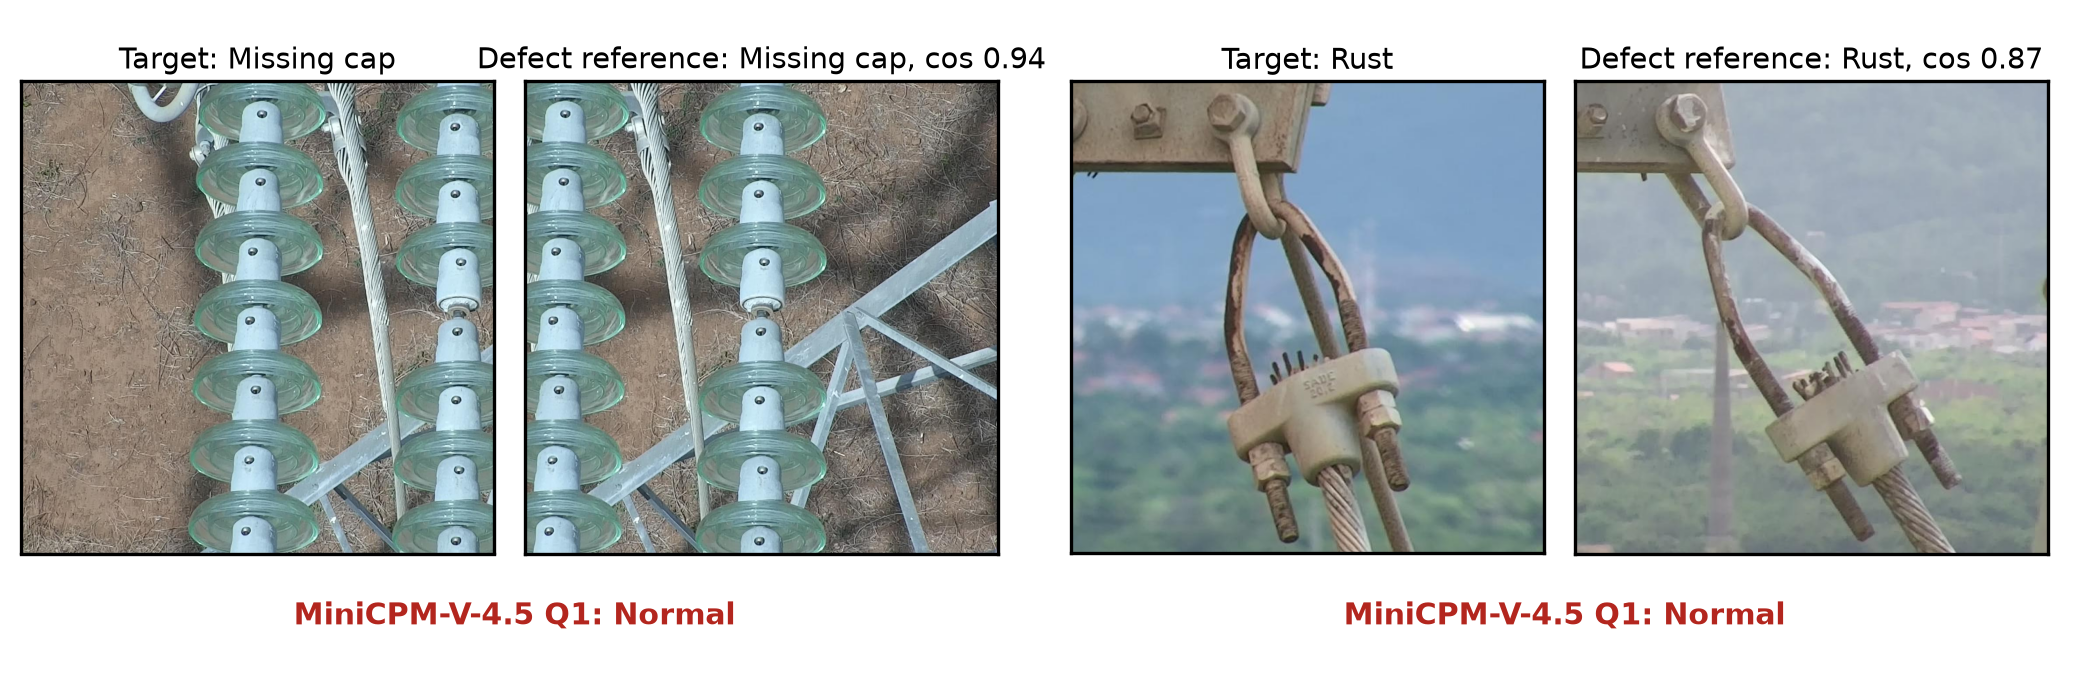
\includegraphics[width=\linewidth]{figures/fig_defect_reference_en.png}
\caption{Two gold targets with their retrieved defect references, which show the same defect type (the missing-cap reference is a neighbouring crop of the same photograph). With this reference MiniCPM-V-4.5 called both targets normal. Images: InsPLAD~\cite{vieira2023insplad}, CC BY-NC 3.0.}
\label{fig:defectref}
\end{figure}

\section{A Question-Independent Verification Agent}\label{sec:agent}
\subsection{Design}
The agent starts from the direct answer with a retrieved (diffdate) normal reference. This \emph{direct} condition differs from the fixed normal reference of Table~\ref{tab:conditions}; with it, InternVL's Q1 F1 is .776 and its balanced accuracy .777. Each question is re-examined on its own: a re-check sees only the reference and target images, the question and that question's own first answer. No other question's answer is shown, used for routing or overwritten. Contradictions between questions are computed only after all final answers are stored (Figure~\ref{fig:agent}). Q1 is never re-checked, because a dev pilot that re-asked every question collapsed InternVL's Q1 F1 from .82 to .08, so Q1 is identical across policies.

\begin{itemize}
  \item \textbf{Q2, verification agent.} A ``second look'' prompt shows the model's own first answer, which may be right or wrong, together with one-sentence visual definitions of the four options.
  \item \textbf{Q2, revised candidate.} A fresh question with revised definitions of all four options (adding rust cues) and no prior answer.
  \item \textbf{Q3.} A separate nine-region-plus-``none'' question is asked for every image. A presence question comes first, and only a positive answer triggers a full-frame $3\times3$ position question. We score Q3 mainly for \emph{region presence} (a region versus ``none''), so a wrong region on a defective image still counts as ``defect present''. Position is scored separately on the 133 defective images that have a location box (113 drawn by hand and 20 from InsPLAD-seg instance labels; six rust images had no locatable defect). A \emph{position hit} means that the reported cell contains the center of one of the image's boxes, the cell rule of our multi-region run (Section~\ref{sec:missing}). We added this position score after the gold run and computed it from the saved answers.
\end{itemize}
\begin{figure}[t]
\centering
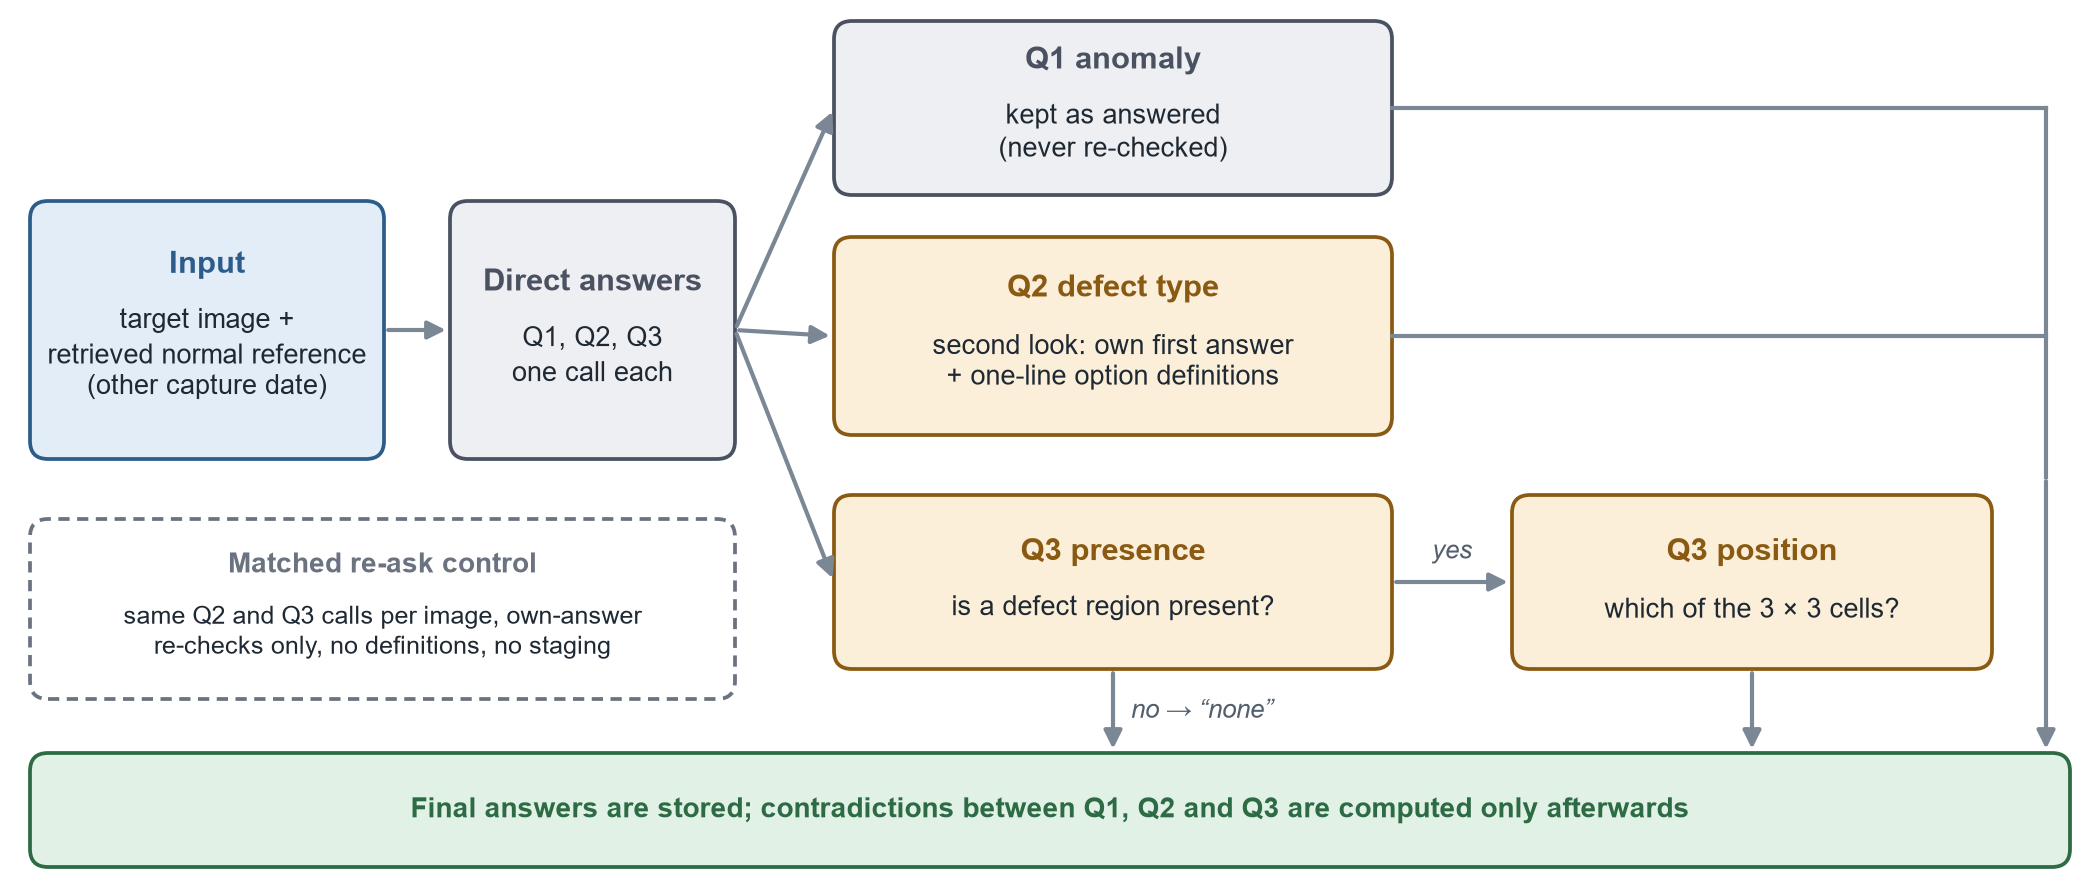
\includegraphics[width=\linewidth]{figures/fig_agent_en.png}
\caption{The question-independent verification agent and the matched re-ask control (Section~\ref{sec:matched}). Each question is re-examined only with its own inputs and its own earlier answer.}
\label{fig:agent}
\end{figure}

The agent and candidate were chosen on dev (the candidate post hoc, from the additional 200 dev images) and run once on gold with InternVL3.5-8B. That run used 1,606 calls (492 direct answers and 1,114 tool calls) with zero errors and zero invalid outputs.

\subsection{Results}
Table~\ref{tab:agent} and Table~\ref{tab:ci} summarize the gold run. Against the direct question, the agent improves Q2 macro-F1 by $+.118$ (95\% CI $[+.043,+.199]$) and the candidate by $+.102$ ($[+.030,+.177]$); Q1--Q2 joint accuracy rises by $+.085$ and $+.093$. Q2 is a four-way question that includes ``normal''. Of the agent's 27 additional correct answers, 23 are on normal images (63 $\rightarrow$ 86). On the 139 defective images, correct types rise only from 93 to 97 for the agent and to 94 for the candidate (Table~\ref{tab:perdefect}). Macro-F1 rises more than these counts suggest for two reasons. Fewer images receive a wrong defect label, which raises the precision of the defect classes; the direct question, for example, calls 43 images without a missing cap ``missing cap'', the agent 17. Bird nests are also recognised more often (7 $\rightarrow$ 19 of 23). The candidate is not distinguishable from the verification agent (Q2 macro-F1 $-.017$, CI $[-.073,+.036]$).

The staged Q3 raises region-presence BAcc by $+.277$ and cuts normal false regions from 93/107 to 16/107. The direct region question, however, reports a region on almost every image: on 93 of the 107 normal images, all 112 rust and bird-nest images and 23 of the 27 missing caps. Its presence BAcc (.551) is therefore barely above that of a constant ``region'' answer (.500). The model's own binary Q1, asked once with the same reference and shared by all policies, is a stricter comparison. Q1 raises 17 false alarms and misses 40 defects; the staged Q3 raises 16 and misses 27, so it is better on both counts. Its large drop in false regions, by contrast, mostly reflects how weak the direct region question is.

Position does not improve. The reported cell is a position hit on 29 of the 133 located defects for the direct question and on 31 for the agent (paired difference $+.015$, CI $[-.045,+.075]$), while answering ``center'' for every image would score 72. Counting only images where a region was reported, the hit rate is 22\% for the direct question and 29\% for the agent. The staging thus removes some wrong cells without placing the remaining ones better.

Relative to the direct question, the agent misses more defects. Defective images judged defect-free rise from 4/139 to 27/139, and the CI of this false-none increase excludes zero ($+.165$, $[+.103,+.234]$). Most of the extra misses are missing caps. The staged Q3 reports a defect region on only 9 of 27 missing-cap images, against 23 for the direct question (bird nests 23$\rightarrow$18 of 23, rust 89$\rightarrow$85 of 89). Because the direct question reports a region almost everywhere, its 23 do not show that the model recognised the caps: Q1 flags only 3 of the 27. Defect typing shows the same weakness (Table~\ref{tab:perdefect}). Normal images and bird nests improve, while rust drops slightly (79$\rightarrow$73 for the agent, 74 for the candidate). Missing caps fall from 7/27 to 5/27 for the agent and to 2/27 for the candidate, which calls 25 of the 27 ``normal''. The additional 200 dev images were used to choose the candidate (Appendix Table~\ref{tab:dev}). On them, the increase in Q3 misses replicates (2$\rightarrow$15 of 99) but the defect-type pattern does not: there the agent and candidate raise missing-cap Q2 from 1 to 5 of 21.

\begin{table}[t]
\centering
\caption{Verification agent on gold v2 (InternVL3.5-8B, 246 images). Direct: the same model with a retrieved (diffdate) normal reference, a different condition from Table~\ref{tab:conditions}. Q1 is asked once and shared by all policies. Q2 is the four-way type question, including ``normal''. Q3 presence counts any reported region as ``defect present''; Q3 position is a post hoc score on the 133 defective images with a location box.}
\label{tab:agent}
\begin{tabular}{lrrr}
\toprule
Metric & Direct & Agent & Candidate \\
\midrule
% Source: gold run ZIP 0c577ffe3bdd (reports/q23_gold_evaluation_2026-10-15), InternVL3.5-8B, L4, 1,606 calls, 0 errors, 0 invalid.
% Columns: metric, direct, verification agent, revised candidate.
Q1 anomaly F1 (fixed in all policies)        & .776 & .776 & .776 \\
Q2 defect macro-F1                           & .522 & \textbf{.640} & .623 \\
Q2 defect balanced accuracy                  & .510 & \textbf{.659} & .639 \\
Q2 correct (/246)                            & 156 & 183 & \textbf{187} \\
Q1--Q2 joint correct (/246)                  & 142 & 163 & \textbf{165} \\
Q1--Q2 consistency error                     & .211 & .167 & \textbf{.150} \\
\midrule
Q3 presence balanced accuracy                & .551 & \textbf{.828} & \textbf{.828} \\
Q3 false region on normal images (/107)      & 93 & \textbf{16} & \textbf{16} \\
Q3 false ``none'' on defective images (/139) & \textbf{4} & 27 & 27 \\
Q1--Q2--Q3 joint correct (/246)              & 91 & 156 & \textbf{157} \\

\bottomrule
\end{tabular}
\end{table}

\begin{table}[t]
\centering
\caption{Paired bootstrap differences (2,000 resamples over images).}
\label{tab:ci}
\begin{tabular}{llrr}
\toprule
Comparison & Metric & $\Delta$ & 95\% CI \\
\midrule
% Source: gold run 0c577ffe3bdd, paired bootstrap over images, 2,000 resamples.
% Candidate rows are the published significance.csv. Agent-vs-direct rows were recomputed on CPU from the saved
% answers.csv with the same repository functions (no new inference); that recomputation reproduces the
% published candidate rows exactly. Q3 is shared by agent and candidate.
% Q3 position row: results/latest/gold_v2_q3_position/significance.csv (133 located defects, seed 42).
% Columns: comparison, metric, difference, 95% CI.
Agent $-$ direct        & Q2 macro-F1                 & $+.118$ & $[+.043, +.199]$ \\
Agent $-$ direct        & Q1--Q2 joint                & $+.085$ & $[+.033, +.142]$ \\
Candidate $-$ direct    & Q2 macro-F1                 & $+.102$ & $[+.030, +.177]$ \\
Candidate $-$ direct    & Q1--Q2 joint                & $+.093$ & $[+.045, +.142]$ \\
Candidate $-$ agent     & Q2 macro-F1                 & $-.017$ & $[-.073, +.036]$ \\
Candidate $-$ agent     & Q1--Q2 joint                & $+.008$ & $[-.028, +.045]$ \\
\midrule
Agent/candidate $-$ direct & Q3 presence BAcc            & $+.277$ & $[+.222, +.328]$ \\
Agent/candidate $-$ direct & Q3 normal false-region rate & $-.720$ & $[-.800, -.625]$ \\
Agent/candidate $-$ direct & Q3 defect false-none rate   & $+.165$ & $[+.103, +.234]$ \\
Agent/candidate $-$ direct & Q3 position hit rate (/133) & $+.015$ & $[-.045, +.075]$ \\

\bottomrule
\end{tabular}
\end{table}

\begin{table}[t]
\centering
\caption{Q2 correct answers per ground-truth class on gold v2. Re-ask: matched-call control (Section~\ref{sec:matched}). Defective: the three defect classes together.}
\label{tab:perdefect}
\begin{tabular}{lrrrrr}
\toprule
Class & Support & Direct & Re-ask & Agent & Candidate \\
\midrule
% Source: q2_by_defect.csv of the matched-call run 902a9f8a1752 (the first three policies equal gold run 0c577ffe3bdd).
% Columns: class, support, direct, matched re-ask, verification agent, revised candidate.
Normal              & 107 & 63 & 86 & 86 & \textbf{93} \\
Rust                & 89  & \textbf{79} & 54 & 73 & 74 \\
Bird nest           & 23  & 7  & 7  & \textbf{19} & 18 \\
Missing cap         & 27  & \textbf{7} & 3 & 5 & 2 \\

\bottomrule
\end{tabular}
\end{table}

\subsection{Structure or more calls? A matched-call control}\label{sec:matched}
Per image, the agent makes two Q2 calls and up to three Q3 calls, where the direct question makes one of each. To test whether the gain is just the extra calls, we add a \emph{matched re-ask} policy. It spends the same Q2 and Q3 calls on every image as the agent but adds neither definitions nor staging. Q2 gets one own-answer re-check without definitions. Q3 gets as many sequential own-answer re-checks as the staged Q3 used for that image. We repeat the shown answer rather than the identical prompt, because the identical prompt under greedy decoding would trivially reproduce the first answer. The agent's saved gold calls are reused, so only the 622 control calls are new. The committed protocol fixed the primary comparison (agent $-$ re-ask, paired bootstrap) before the run. We read a CI that excludes zero as evidence that the gain is not explained by additional calls.

\begin{table}[t]
\centering
\caption{Matched-call control on gold v2. Calls/img counts Q2 and Q3 calls (Q1 is shared). The matched re-ask spends identical calls to the agent on every image (Q2 492, Q3 622 in total) but adds no definitions or staging.}
\label{tab:matched}
\begin{tabular}{lrrrrr}
\toprule
Policy & Calls/img & Q2 F1 & Q3 pres.\ BAcc & Normal FP & Defect FN \\
\midrule
% Source: gold_matched_call_results.zip sha256 902a9f8a1752... (reports/gold_matched_call_evaluation_2026-10-23),
% InternVL3.5-8B, NVIDIA L4, main@36458d5, 622 new calls + 1,606 reused, 0 errors, 0 invalid. CPU audit: audit_summary.json.
% Columns: policy, Q2+Q3 calls per image, Q2 macro-F1, Q3 presence BAcc, normal false region (/107), defect false none (/139).
Direct                           & 2.00 & .522 & .551 & 93 & \textbf{4} \\
Matched re-ask                   & 4.53 & .476 & .625 & 74 & 8 \\
Verification agent               & 4.53 & \textbf{.640} & \textbf{.828} & \textbf{16} & 27 \\
Revised candidate                & 3.53 & .623 & \textbf{.828} & \textbf{16} & 27 \\
\midrule
\multicolumn{6}{l}{Agent $-$ re-ask: Q2 macro-F1 $+.164$ $[+.093, +.242]$; Q3 presence BAcc $+.203$ $[+.145, +.257]$} \\
\multicolumn{6}{l}{Re-ask $-$ direct: Q2 macro-F1 $-.046$ $[-.095, +.000]$; Q3 presence BAcc $+.074$ $[+.025, +.124]$} \\

\bottomrule
\end{tabular}
\end{table}

The control ran on the same GPU type (L4) with 622 new calls, 0 errors and 0 invalid outputs. The three published policies, recomputed from their reused calls, are unchanged. The agent outperforms the equal-call re-ask by $+.164$ Q2 macro-F1 (95\% CI $[+.093,+.242]$) and $+.203$ Q3 presence BAcc ($[+.145,+.257]$) (Table~\ref{tab:matched}). Additional calls therefore do not explain the gain; it depends on what the agent adds, namely option definitions for Q2 and presence-then-position staging for Q3. The control removes both at once, so it cannot separate the information in the definitions from the effect of the staging.

Re-asking alone does not help Q2 ($-.046$, $[-.095,+.000]$). It mainly pushes answers towards ``normal'': ``normal'' predictions rise from 86 to 139 of 246. That repairs 30 normal images but breaks 26 rust images, 21 of which become ``normal''; Table~\ref{tab:perdefect} shows the net per-class result. On Q2 false alarms, re-asking alone already matches the agent: both label 21 of 107 normal images with a defect type. The agent moves in the same direction less strongly (117 ``normal'' predictions). Its definitions hold rust at 73/89 (re-ask: 54) and recover bird nests (7 $\rightarrow$ 19/23). For Q3, re-asking gives a small presence gain ($+.074$, $[+.025,+.124]$) with a matching small shift: normal false regions 93 $\rightarrow$ 74 and missed defects 4 $\rightarrow$ 8; position hits are 30 of 133 (direct 29). The staged presence question amplifies both effects. Compared with the re-ask, it removes many more false regions ($-.542$ in rate, $[-.636,-.447]$) and misses more defects ($+.137$, $[+.079,+.201]$). Missing caps account for most of this gap: the re-ask still reports a region on 20 of 27 of them, the staged agent on 9. Asking again already makes the model somewhat more conservative, and the agent's additions turn that shift into a large net gain while enlarging the miss rate.

\section{Why Missing Components Are Missed}\label{sec:missing}
No question detects missing caps reliably. On gold, Q1 flags 3 of the 27, Q2 names the defect in 7 (direct), 5 (agent) and 2 (candidate), and the staged Q3 reports a region on 9. The direct region question reports one on 23, but it also does so on 87\% of normal images. A separate multi-region run on gold, whose direct question was less biased (29 of 107 normal false alarms), asked for every defect cell with fixed references; it missed 25 of the 27 caps with both direct and staged prompting. All 27 gold cases are glass insulators, an asset with only five gold normals, so asset and defect effects are confounded. We studied missing caps on development data only, never gold. Dev240 contains 25 of them, of which 4 fall in the 40-image design subset used for most model swaps. Each intervention used fixed settings, and where a pass criterion was defined it was written before the run. One exception: the cross-model re-check was re-run once with a changed proposal format after invalid outputs (Appendix Table~\ref{tab:negative}).
\begin{itemize}
  \item \textbf{Input and wording.} Doubling the target's visual tiles, short defect-evidence prompts, and both together all reduced missing-cap recall on dev240 against the revised-definition Q2 control. Recall fell from 6/25 to 2, 4 and 1 of 25 respectively.
  \item \textbf{Other models and detectors.} Swapping in Qwen3-VL-8B or Ovis2.5-9B for Q2 recovered none of the 4 design-subset missing caps (1 $\rightarrow$ 0 for both). As the Q3 presence model, Qwen3-VL cut missing-cap misses on dev240 only from 10 to 8 of 25 while adding other errors. Three anomaly detectors used for Q3 presence (AdaCLIP, AnomalyVFM, InCTRL) all lowered presence BAcc.
  \item \textbf{Part evidence.} Three tools failed their predeclared reliability gates on normal glass insulators (6 of 7 needed): open-vocabulary detection with Grounding DINO (3 of 7), counting with CountGD++ (2 of 7) and SAM masks (4 of 7). SIFT registration passed its synthetic controls but aligned 0 of 8 real reference--target pairs. DIFT correspondence passed 0 of 7 known-flip checks. None could serve as part-count evidence.
  \item \textbf{Crops of the location.} The model was shown crops of three kinds (20 positive images each): the candidate cell, the human-annotated cell and the annotated box. InternVL answered ``no region'' in all 60 calls, but this prompt also showed the model's earlier empty answer. A separate question without that cue asked only whether a component is missing or broken, and the model answered ``absent'' in all 60 calls. Only positive images were tested.
  \item \textbf{A supervised expert.} We trained a frozen DINOv2 feature plus a logistic head on glass-insulator train labels, using date-disjoint internal splits. The dev images may share capture dates with training. The head detected 25 of 25 dev missing caps with 1 false alarm on 25 dev normals; its normal false-alarm rate on the date-disjoint internal test was 13.8\%. Given to the LVLM as a suggestion to re-check, it raised dev missing-cap Q2 from 6 to 14 of 25, against 8 for a matched re-ask. This breaks the training-free premise and covers one asset only. Occlusion analysis of the head placed the exact grid cell in 12 of 24 cases, against 8 of 24 for a fixed center guess (paired CI includes zero). Integrated gradients~\cite{sundararajan2017ig} scored at most 9 of 24. With 32 integration steps, however, 49 of 52 maps failed the completeness check, so this test of IG is inconclusive.
\end{itemize}
In summary, training-free changes to input, wording, model or added tools did not make the 8B LVLM register missing caps, even with the region cropped for it. Explicit evidence from a supervised classifier did change its answers. We read this as a perception limit for this defect type, which prompts and routing still modulate: on gold, the agent's own definitions and staging lowered missing-cap answers.

\section{Discussion and Limitations}
\paragraph{What the agent changes.} The verification agent makes the model more conservative. The matched-call control shows that part of this conservatism comes simply from asking again~\cite{huang2024cannotselfcorrect}, and the agent's definitions and staging channel it into a real gain. Compared with the direct region question, the agent removes most false alarms on normal images and misses more defects. That trade-off is partly a property of the comparison: the direct question reports a region on almost every image, so almost any answer that discriminates would remove false alarms and add misses relative to it. Against the model's own binary question the staged answer is better on both counts. Most of the agent's additional correct Q2 answers are on normal images, and it does not locate defects better. Single summary scores hide such distinctions. Benchmarks should report the normal false-alarm rate and per-class recall alongside macro-F1, and compare each answer with constant baselines.

\paragraph{What we propose.} Missing components are the main risk. On gold the staged Q3 answered ``no region'' on 27 defective images, 18 of them missing caps. A missing component can lead to a line failure, while a false alarm costs a second look, so we do not recommend using the agent's ``no defect'' as a final decision. Our data suggest three directions.
\begin{itemize}
  \item \textbf{Reviewing ``no defect'' answers.} Because the direct question almost always reports a region, the 102 images (41\%) on which it disagrees with the staged Q3 are nearly the same as the 118 (48\%) on which the agent answers ``no region''. If a human reviews the 102 and is right, misses fall from 27 to 3 (all missing caps); reviewing all 118 removes every miss. Either way 16 false alarms remain. Disagreement therefore adds little over reviewing every ``no defect'' answer, and both rules send close to half of the images to a person. We computed this post hoc on gold to illustrate the idea and did not tune a review rule. A cheaper filter would need a signal that registers missing caps, and none of the LVLM answers provides one.
  \item \textbf{Explicit evidence for absence defects.} Prompts, crops and other LVLMs did not make the model register missing caps, but an asset-specific supervised head detected all 25 dev missing caps, and its suggestion changed the LVLM's answers (Section~\ref{sec:missing}). A hybrid in which a small supervised detector can veto ``normal'' for high-risk classes trades the training-free premise for safety.
  \item \textbf{Reporting misses explicitly.} Macro-F1 and joint accuracy rose while missing-cap detection fell. Per-class recall, recall at a fixed normal false-alarm rate, or a cost-weighted score would expose such a shift.
\end{itemize}
Whether larger LVLMs show the same trade-off is open; we tested only 4--8B open models.

\paragraph{Limitations.} (1) The agent was evaluated with one model (InternVL3.5-8B), so transfer to other models is untested. (2) Gold has 246 images and prior exploratory use, and dev was explored repeatedly, so dev gains are exploratory. (3) Missing caps occur in one asset only, which confounds defect and asset. (4) Position is weak and its labels are coarse. On the 133 located defects the agent's reported cell is a hit on 31 (direct question 29), and in the multi-region run the exact cell set matched on 12 of 133 with either prompt. A constant ``center'' answer scores 72 and 46 on these two measures. One cell per box center under-describes large or spread defects. (5) Vision-expert scores are transductive percentiles. (6) No new untouched holdout exists, because the Aligned Core's defective images are all in gold. Unused defective images remain only in supervised train. (7) MiniCPM-V-4.5's 20 vision-expert configurations come from sampled decoding. Its baseline and reference rows were re-run greedily.

\section{Conclusion}
InsPLAD-QA provides a hash-aligned, manually reviewed benchmark for LVLM power-line inspection with a shared prompt, schema and evaluator. Normal references raise anomaly-detection F1, but balanced accuracy rises clearly only for InternVL3.5-8B and Qwen3.5-4B and falls for MiniCPM-V-4.5, and their effect on coherence is mixed. Anomaly-detector cues trade anomaly detection for defect typing. A question-independent verification agent improves the four-way type answer, although most of its additional correct answers are on normal images. Its staged region-presence answer has fewer false alarms and fewer misses than the model's own binary answer, while the direct region question it replaces reports a region almost everywhere; it does not improve position. An equal-call re-ask does not reproduce the gain, which therefore comes from the agent's definitions and staging. No question detects missing caps reliably. On development data, none of the training-free interventions we tried recovered them, and InternVL3.5-8B did not report them on crops of the annotated location.

\bibliographystyle{unsrtnat}
\bibliography{refs}

\appendix
\section{Additional development images}
\begin{table}[h]
\centering
\caption{The additional 200 dev images (used to choose the gold candidate). ``Revised'' uses the revised Q2 together with a review-stage Q3 that was rejected and never run on gold. Only its Q2 value corresponds to the gold candidate.}
\label{tab:dev}
\begin{tabular}{lrrr}
\toprule
Metric & Direct & Agent & Revised \\
\midrule
% Source: reports/q2_q3_refined_evaluation_2026-10-14/d348a43771e9 (dev, additional 200 images not used for design).
% Columns: metric, direct, verification agent, revised.
Q2 macro-F1                          & .514 & .654 & \textbf{.698} \\
Q3 presence balanced accuracy        & .559 & \textbf{.810} & .759 \\
Q3 false region on normal (/101)     & 87 & 23 & \textbf{19} \\
Q3 false ``none'' on defective (/99) & \textbf{2} & 15 & 29 \\

\bottomrule
\end{tabular}
\end{table}

\section{MiniCPM-V-4.5: greedy versus sampled decoding}
\begin{table}[h]
\centering
\caption{MiniCPM-V-4.5 on gold v2, greedy re-run / published sampled run (temperature 0.7). Same prompts, images and references; 2,136 greedy calls, 0 errors, 0 invalid outputs. Greedy Q1 balanced accuracy: image-only .656, normal .587, defect .494, both .645.}
\label{tab:minicpm}
\small
\begin{tabular}{lrrrrr}
\toprule
Condition & Q1 F1 & Q2 F1 & Joint & CE & FDR \\
\midrule
% Source: MiniCPM-V-4.5 greedy re-run 1661680ed362 (L4, main@49059c6, 2,136 calls, 0 errors, 0 invalid) vs the
% published sampled values (results/latest/gold_v2_consistency_metrics). CPU audit: audit_summary.json.
% Columns: condition, then greedy / sampled for Q1 F1, Q2 macro-F1, joint, consistency error, false defect rate.
\CondImg  & .618 / .583 & .483 / .450 & .496 / .431 & .280 / .341 & .308 / .411 \\
\CondNorm & .753 / .752 & .461 / .469 & .484 / .480 & .110 / .126 & .841 / .841 \\
\CondPos  & .014 / .000 & .328 / .332 & .415 / .415 & .142 / .146 & .047 / .047 \\
\CondBoth & .648 / .632 & .488 / .500 & .447 / .439 & .301 / .317 & .607 / .589 \\

\bottomrule
\end{tabular}
\end{table}

\section{Negative follow-up experiments}
\begin{table}[h]
\centering
\caption{Follow-up interventions for missed defects (development data only; fixed settings; pass gates where defined).}
\label{tab:negative}
\small
\begin{tabular}{p{4.3cm}p{2.2cm}p{6.8cm}}
\toprule
Intervention & Data & Result \\
\midrule
Target zoom $\times$ short prompt (2$\times$2) & dev 240 & Q2 F1 .693 $\rightarrow$ .594/.627/.593; missing caps 6 $\rightarrow$ 2/4/1 of 25 \\
Cross-model re-check (InternVL+Qwen) & dev 40 & Q2 F1 .652 $\rightarrow$ .692, CI $[-.055,+.181]$; format revised once after invalid outputs; additional-200 run excluded (invalid outputs) \\
Qwen3-VL-8B replacement & dev 40 $\rightarrow$ 240 & Q3 BAcc .792 $\rightarrow$ .833 on 40 not reproduced on 240 (.818 $\rightarrow$ .754); Q2 missing caps 1 $\rightarrow$ 0 of 4 \\
Ovis2.5-9B for Q2 & dev 40 & Q2 F1 .652 $\rightarrow$ .637; missing caps 1 $\rightarrow$ 0 of 4 \\
AdaCLIP / AnomalyVFM / InCTRL for Q3 presence & dev 40 & BAcc .792 $\rightarrow$ .667 / .479 / .531 \\
AnomalyR1 & smoke 5 & comparison model invalid 2/10; not comparable \\
Grounding DINO / CountGD++ / SAM part evidence & glass insulators & reliability gates failed (e.g.\ CountGD repeatability 2/7, SAM 4/7, need 6/7) \\
SIFT registration / DIFT correspondence & 8 ref--target pairs / 7 normals & 0/8 real pairs aligned; 0/7 flip checks \\
Crops: candidate cell / annotated cell / annotated box & dev 20 & 0/20 recovered in each arm (prompt showed the earlier empty answer) \\
Independent presence question & dev 20 & 60/60 calls answer ``absent'' \\
Supervised missing-cap head (frozen DINOv2) & dev 50 glass & presence 25/25 (1/25 normals flagged); location exact 12/24 vs.\ center 8/24 \\
Integrated-gradients localization & dev 24 & exact $\le$ 9/24; completeness warnings 49/52 (inconclusive) \\
\bottomrule
\end{tabular}
\end{table}

\section{Reproducibility}
Code, prompts, frozen configurations, Colab notebooks, leaderboards and per-question answers for the main results are in the project repository, together with a summary of every follow-up run. Some dev follow-ups in Appendix Table~\ref{tab:negative} (the other LVLMs, anomaly detectors, cross-model re-check and part-evidence and alignment probes) ran from frozen source bundles; their code is archived rather than in the repository. Raw per-call logs (prompts, outputs, latencies) and all of this archived code are kept with SHA-256 hashes and available on request. Runs record the model ID, backend, benchmark commit, protocol and status; the later runs (agent, matched-call, MiniCPM re-run) also record the GPU. Notebooks verify the exact code revision before inference and resume from checkpoints saved every 20 calls. InsPLAD images are used under the dataset's CC BY-NC 3.0 license; Figures~\ref{fig:pipeline}--\ref{fig:agent} are generated by \texttt{make\_figures.py} from the released result files.

\end{document}
